
\documentclass[12pt]{article}

\usepackage{sbc-template}
\usepackage{graphicx,url}
\usepackage{array}
\usepackage{color}
\usepackage{listings}
\usepackage{fancyhdr}
\usepackage[T1]{fontenc}
\usepackage{epsfig}
\usepackage{rotating}
\usepackage{setspace}

\usepackage{graphicx}

\usepackage[square,
            authoryear,
            sort&compress,]{natbib}
\let\cite=\citep

%\usepackage[brazilian]{babel}
\usepackage[latin9]{inputenc}

     
\sloppy
\newcommand{\papertitle}{KDM-RE: A Model-Driven Refactoring Tool for KDM}
\title{\papertitle}

\author{Rafael S. Durelli\inst{1,3}, M\'{a}rcio E. Delamaro\inst{1} and Valter V. de Camargo\inst{2}}

 
\address{Computer  Systems Department University of S\~{a}o Paulo\\
  S\~{a}o Carlos, SP, Brazil.
\nextinstitute
  Computing Departament\\ Federal University of S\~{a}o Carlos (UFSCAR)\\
  S\~{a}o Carlos, SP, Brazil.
\nextinstitute
  RMoD Team, INRIA, Lille, France
  \email{\{rdurelli, delamaro\}@icmc.usp.br\inst{1}, valter@dc.ufscar.br\inst{2}}
}

\begin{document} 

\maketitle

\begin{abstract}



%ABSTRACT defined by Valter

Architecture-Driven Modernization (ADM) it is a new proposal defined by OMG which advocates to apply Model-Driven Modernization (MDD) to legacy system. Its main metamodel is KDM, which is language and platform independent and allows representing various artifacts of a system at different abstraction levels. For this type of modernization be adequately done, model-driven refactoring need to be developed. However, there is a lack in the literature of tool to lead modernizer engineer to apply refactorings in the KDM metamodel, which complicates the modernization task. To fulfill this lack, in this paper it is described a tool, that implements 17 fine-grained refactorings proposed by Fowler in KDM's instances. In order to provide support to the modernizer engineer, these instances can be visualized as UML class diagrams. Therefore, the modernizer engineer can detect 
"model smells" in these diagrams and apply the refactorings.




%ABSTRACT 1
%Software refactoring is a proven technique that aims at improving the quality of source code.
 %However, with the advent of Architecture-Driven Modernization (ADM) and its meta-model - Knowledge Discovery Metamodel (KDM), it seems a good alternative for shifting from source-code refactoring to model-driven refactoring. The main goal of this shift is to create a language and platform independent catalog of refactoring. 
%Nevertheless, although ADM provides the process for refactoring legacy systems by using KDM, there is a lack of an Integrated Development Environments (IDEs) to lead engineers to apply refactorings as such exist for other object-oriented languages.
%To fulfill this lack herein we describe a tool, implemented as an Eclipse \textit{plug-in}. 
%This \textit{plug-in} supports 17 well known refactorings that are adapted to KDM. It also provides a mechanism to synchronize both the underlying source code and a class diagram after one applies all refactorings into the KDM.

%These refactorings are heavily inspired by well known refactorings in the literature. All refactorings were adapted in order to be applied into KDM models and yet keeping them in synch with the underlying source code as well as a class diagram. 
%Our tool involves three steps: (\textit{i}) reverse engineering, (\textit{ii}) refactoring by means of KDM,
 %and (\textit{iii}) forward engineering. 
%The first step relies on transforming the source code into a KDM's instance. 
%The second step relies on applying refactorings into the KDM's instance. 
%The third step consists of generating the refactored source-code.


%ABSTRACT 2
%Refactoring is recognized as an essential practice in the context of evolutionary and agile software development.
%Nowadays, with the advent of Architecture-Driven Modernization (ADM) it has become a good alternative for refactoring systems in a Model-Driven Architecture (MDA) way by using its metamodel - Knowledge Discovery Metamodel (KDM). Nevertheless, although ADM provides the process for refactoring legacy systems by means of KDM, is so far missing an Integrated Development Environments (IDEs) to lead engineers to automatically apply refactorings as such exist in others object-oriented languages. We describe a tool, implemented as an Eclipse \textit{plug-in} designed to fulfill exactly this need. This tool supports 16 refactorings that are heavily inspired by refactorings well known in the literature. Our tool involves three steps: (\textit{i}) reverse engineering, (\textit{ii}) fully automated application of the refactoring by means of KDM, and (\textit{iii}) forward engineering. The first step relies on transforming the source code into a KDM's instance. The second step relies on applying refactorings into the KDM's instance. The third step consists of generating the refactored source-code.

\end{abstract}
\section{Introduction\label{sec:introduction}}
 Model-driven software engineering (MDSE) is becoming the most promising paradigms in software engineering. MDSE promotes the use of models as key artifacts in all phases of the software development lifecycle. Out of the many approaches to model-driven engineering, the Architecture-Driven Modernization (ADM) which has been proposed by OMG (Object Management Group) and advocates conducting refactoring following the principles of MDA (Model-Driven Architecture)~\cite{Ulrich:2010:IST:1841736} has become a great candidate since it aims to promote \textit{(i)} portability, \textit{(ii)} interoperability and \textit{(iii)} reusability. According to the OMG the most important artifact provided by ADM is the KDM metamodel, which is a vertical and horizontal standard metamodel that represents all elements of the existing information  technology architectures. KDM is structured in a hierarchy of four layers; \textit{Infrastructure Layer}, \textit{Program Elements Layer}, \textit{ Runtime Resource Layer} and \textit{Abstractions Layer}. We are specially interested in the \textit{Program Elements Layer} because it defines the ``Code'' packages which is widely used by our tool. The ``Code'' package defines a set of metaclasses that represents the common elements in the source code supported by different programming languages such as: (\textit{i}) ``ClassUnit'' and ``InterfaceUnit'' which represent classes and interface, respectively, (\textit{ii}) ``StorableUnit'' which illustrates attributes and (\textit{iii}) ``MethodUnit'' to represent methods. 

On the other hand, refactoring has been known and highly used both industrially and academically. It is a form of transformation that was initially defined by Opdyke [ref] in the discipline of Object Oriented (OO) Programming as ``a change made to the internal structure of the software while preserving its external behavior at the same level of abstraction''. Nowadays it is possible to identify several catalogs of refactoring for different languages. The most complete and influential was published by Fowler in [6] for refactoring of Java code. 
However, while software reengineers would greatly benefit from the possibility to assess different choices, in practice they mostly rely on experience or intuition because of the lack of approaches providing comparison between possible variations of a change. 
Therefore, software reengineers do not have the possibility to easily apply analyses on different source-code version branches of a system and compare them to pick up the most adequate changes. In this context, the motivations for moving from software refactoring  to model refactoring are: 
(\textit{i}) a model provides an abstract view of the system, hence, visualizations of the structural changes required are easier, 
(\textit{ii}) problems uncovered at the design-level can be improved directly on the model and 
(\textit{iii}) using refactoring in high abstract level can allow the software engineer to explore alternate design paths in much cheaper than software refactoring.

To overcome the described problems, we devised a \textit{plug-in} on the top of the Eclipse Platform named KDM-RE (\textbf{K}nowledge \textbf{D}iscovery \textbf{M}odel-\textbf{R}efactoring \textbf{E}nvironment). Firstly, this \textit{plug-in} provides a model-driven refactoring based on KDM models. Secondly, it also supplies a multiple versions of a system at level models (KDM), enabling to the engineer  to work interactively on multiple models and to explore alternate refactoring path. Finally, after the best alternate refactoring path is chosen by the engineer, a forward engineering is performed and the source code of the refactored target system is generated again. Notice that KDM-RE supports 16 refactorings that are heavily inspired by the refatorings given by Fowler~\cite{aqui}. These refactorings are split up into three groups. The first group named \textbf{Moving Features Between Objects} which consists of relatively simple refactorings such as moving and creating features. The second group called \textbf{Organizing Data} is a set of refactorings to be applied in order to make working with data easier. The third group is named \textbf{Dealing With Generalization} and it represents refactorings to mostly dealing with moving methods and fields around a hierarchy of inheritance. This paper is organized as followed: Section 2 provides information related to KDM-RE - Section 3 the architecture of KDM-RE is depicted - in Section 4 there are related works and in Section 5 we conclude the paper with some remarks and future directions.







%\section{Motivation\label{sec:motivation}} 
% The motivation is the following: (\textit{i}) there is neither a repository, in which the CFs/CFFs can be stored by domain engineer in order to share it, nor an infrastructure where the CFs can be reused as easy as possible in order to disseminate them; (\textit{ii}) most of the CFs found apply white-box reuse strategies - thus it is important provides a way to assist the instantiation of these CFs using models.     

%(\textit{i}) provide an infrastructure to support the reuse of CFs, (\textit{ii}) allowing application engineers to download CF members to be reused in their applications and (\textit{iii}) allowing application engineers to conduct the reuse of CFs in a model-based fashion.  


%In the literature, it is possible find out a large number of researches related to CFF (COLOCAR REF). In these researches a large number of CFF have been devised (e.g., Security, Persistence, Distribution, etc). Thus, it is important develop an environment in which allows engineers share, manage, and provide full cycle of reuse of these CFF. It is also important supplies a graphical way to allow the engineer examines and reuses the features available in one CFF. For instance, the engineer could reuse piece of code of the CFF just selecting a set of features through a feature model.

%Therefore, this environment would increases the quality of the base applications that are developed in terms of modularity, reuse, maintainability. The efficiency will be achieved through the use of techniques related to reuse of analysis, design and code. The quality of the final applications must also be improved with the reuse, since the artifacts have already been tested and approved.  


%For instance, one engineer has developed a CFF and would like to share it in oder to let another engineer reuse his CFF.  CFF has beed developed and  engineer developed a CFF Moreover, it is also important supplies a graphical way to allow the engineer examines and reuses the features available in one CFF. For instance, the engineer could reuse piece of code of the CFF by selecting a set of features in a feature model. % if them fulfill the base application.  the features available fulfilled the base application the engineer would reuse such features.  %whether the features available in one CFF fulfill the base application requirements. 
%To the best of our knowledge there are neither an approach nor a tool with these functionality. In order to overcome such limitations we have put forward a plug-in, in which is described in the next sections.	 

%However, to the best of our knowledge, there is neither an approach nor a tool that allows share, management and also provides full cycle of reuse of the CFF. Moreover, it is important a tool that supplies a graphical way to allow the engineer examines previously if the features available in one CFF fulfill the application requirements. %Moreover, it is important that there is way to allow the engineer verify whether the variability/features available in the CFF meet the application requirements that must be developed.  

%Afterwards, the features have been examined and chosen by the engineer it is likewise important provides a way to download only the artifacts that have been chosen.    

%Thus, the CFF can be used during a development process easier and can be provided major computer support to facilitate such as task.     

%It is important that there is a way to examine whether the variability / features available in the family of FTs meet the application requirements that must be developed. In order for families of FTs to be properly used during a development process, and a major computer support to facilitate this task.


% which implements complete cycle of reuse of the CFF. 
%\textbf{Using this plug-in the CFF can be reused in a controlled way. Thus, during the reuse to increase the quality of the developed applications. Furthermore, any manipulation in the CFF can be made through the intermediary of models, so we intend to raise the level of abstraction in which the engineer works.}


%Thus, the objective of this paper is describes this plug-in. 

%Embora v�rios autores j� tenham trabalhado com FTs (Couto et al., 2005; Hanenberg et al., 2004; Huang et al., 2004; Shah e Hill, 2004; Constantinides e Elrad, 2001; Pinto et al., 2002; Rashid e Chitchyan, 2003; Soares et al., 2006; Vanhaute et al., 2001; Huang et al., 2004; Mortensen e Ghosh, 2006a; Mortensen e Ghosh, 2006b; Soares, 2004), n�o � encontrado na literatura o projeto de um reposit�rio de FTs e t�cnicas para busca de um determinado FT que atenda aos requisitos de uma aplica��o. � importante que exista uma forma de averiguar se as variabilidades/caracter�sticas dispon�veis na fam�lia de FTs atendem aos requisitos da aplica��o que deve ser desenvolvida. Para que fam�lias de FTs sejam adequadamente usadas durante um processo de desenvolvimento, � importante um apoio computacional que facilite essa tarefa.

\section{KDM-RE\label{sec:KDM-RE}} 
Figure~\ref{fig:process} depicts the overall process to use KDM-RE - which was adapted based on the horseshoe modernization model. 
It is split into three steps, they are: 
(\textit{i}) reverse engineering, 
(\textit{ii}) refactorings, and 
(\textit{iii}) forward engineering. 
Furthermore, these steps were divided into six levels, as can be seen in Figure~\ref{fig:process} - more details about these steps and its levels are described in next sections:

\begin{figure}[!ht]
\centering
  % Requires \usepackage{graphicx}
  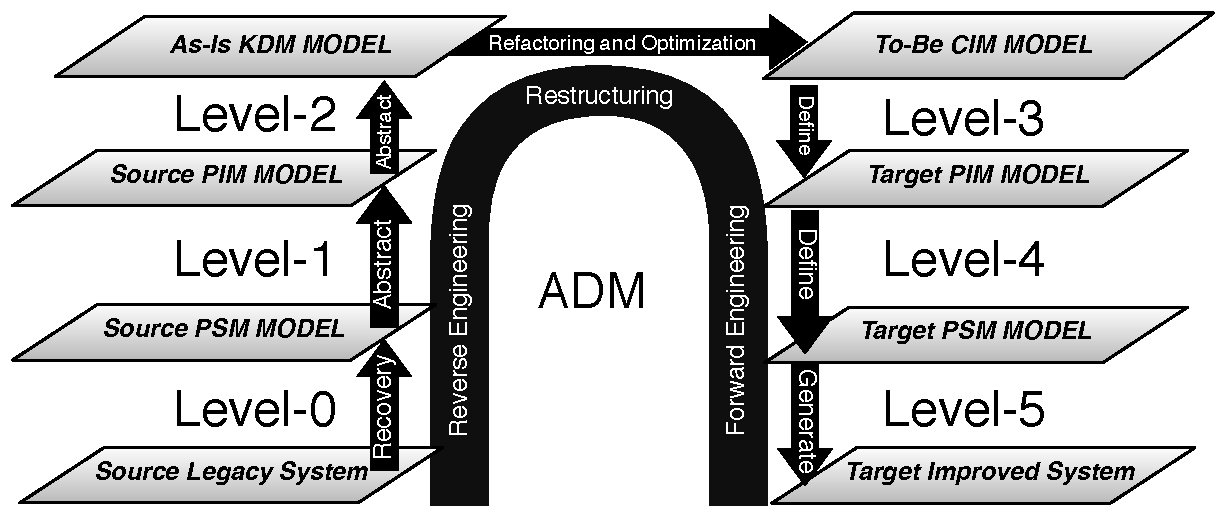
\includegraphics[width=11cm, height=3.8cm]{figure/processoDaFerramenta}
\caption{KDM-RE Process}
\label{fig:process}
\end{figure} 

\subsection{Reverse Engineering}

Herein the engineer provides a KDM file or a source-code from a legacy system. If the source code is the input, then the engineer starts the process in the \textbf{Level-0} by choosing an eclipse project which contains the source-code to realize the refactorings.  
After that, into \textbf{Level-1} the source-code need to be transformed into a Platform-Specific Model (PSM). 
This PSM is an instance of the source-code which represents all abstraction of the source-code. To realize this transformation we implemented a model extractor in Java. 
Figure~\ref{fig:discovery_java_model} illustrates how KDM-RE manages to assist the engineer to get the instance of this PSM. Figure~\ref{fig:discovery_java_model} (a) shows the eclipse project selected by the engineer - then after the engineer click in a popup menu named ``Discovery Java Model'' the Figure~\ref{fig:discovery_java_model} (b) is shown an excerpt to indicate the correspondence with the legacy Java Model. For instance, each ``Class'' found in the source-code an instance of the meta-classe \texttt{ClassDeclaration} is created, similar each ``Methods'' declarations are transformed to instances of the meta-classe \texttt{MethodDeclaration}, and ``attributes'' are transformed into instances of \texttt{FieldDeclaration}, etc.
%This PSM is an Abstract Syntax Tree (AST) that represents the syntactic struct of Java source code.



After creating the PSM the next level (\textbf{Level-2}) consists in transforming the PSM to a Platform-Indented Model (PIM) which is based on the KDM. 
In this level the KDM-RE uses MoDisco\url{http://www.eclipse.org/MoDisco/} which provides an extensible framework to transform a specific PSM to KDM models in order to represent the systems ``AS-IS''. We added in KDM-RE a popup menu named ``Discovery KDM Model'' which by clicking on it the KDM-RE calls the MoDisco API to get a instance of the KDM based on the earlier PSM.
In Figure~\ref{fig:discovery_java_model}(c) shows how the Java Model is transformed to KDM.
%
\begin{figure}[!ht]
\centering
  % Requires \usepackage{graphicx}
  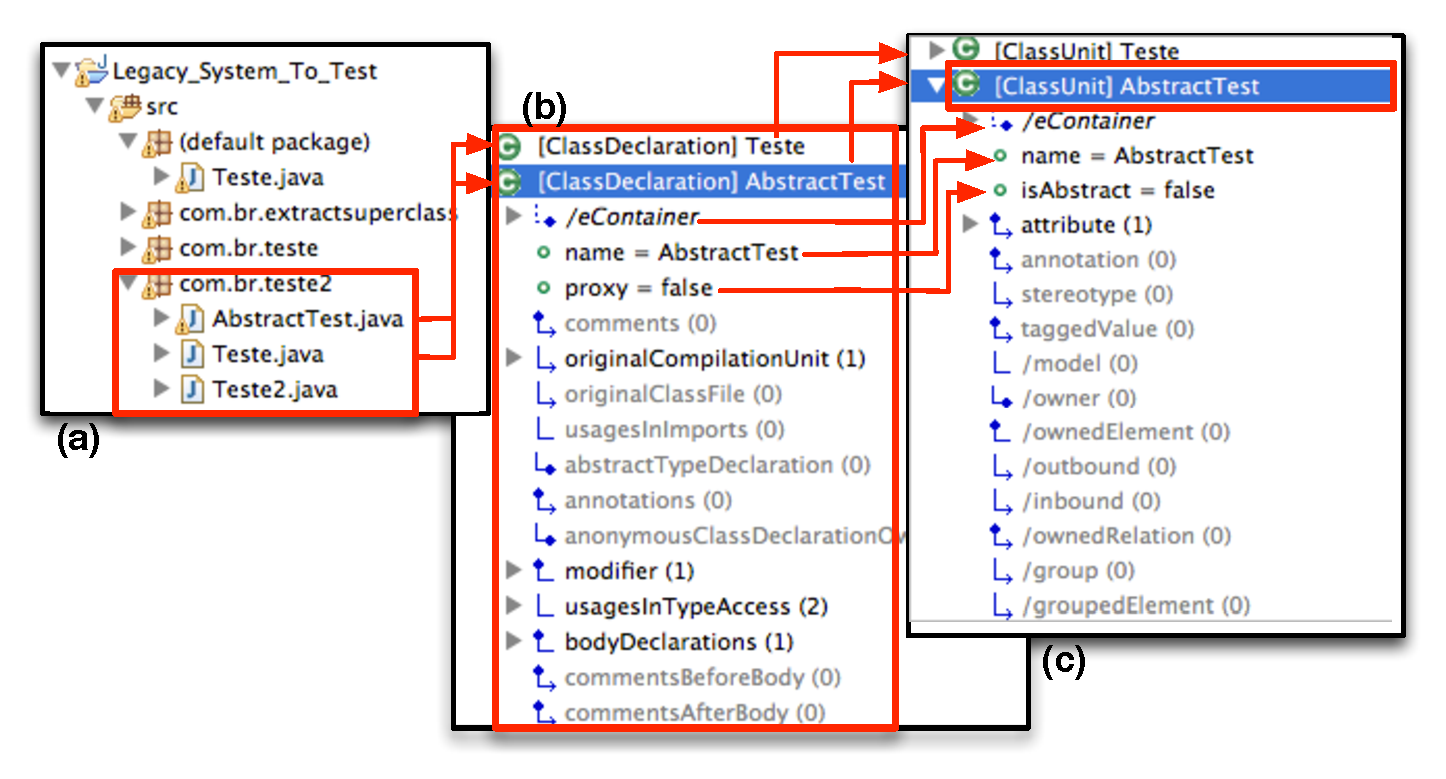
\includegraphics[width=13cm, height=6cm]{figure/GerandoTODOS}
\caption{Process to Discovery Java and KDM Model}
\label{fig:discovery_java_model}
\end{figure}
%
In Figure~\ref{fig:interface} we depicted the main window of our \textit{plug-in}. 
For explanation purpose, we have identified main regions, i.e., \textcircled{a}, \textcircled{b}, \textcircled{c} and \textcircled{d}.

\begin{figure}[!ht]
\centering
  % Requires \usepackage{graphicx}
  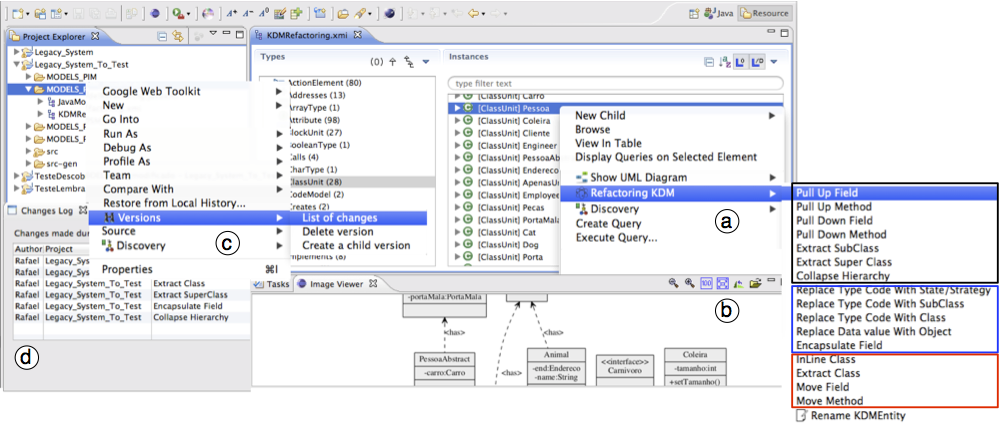
\includegraphics[width=15cm, height=6.8cm]{figure/ScreenShot_tool}
\caption{KDM-RE's Interface}
\label{fig:interface}
\end{figure}

All refactorings provided by KDM-RE are based on the KDM model. 
%Thus, suppose that a KDM model has already been instantiated. 
%All the steps to how obtain a KDM instance are explained further. 
In order to assist the refactorings we extended the KDM's model browser provided by MoDisco. 
We added a popup menu named ``Refactoring KDM'' in this model browser, see Figure~\ref{fig:interface}\textcircled{a}.
By using this menu the engineer can interact with the KDM model and choose which refactoring must be carried out in the KDM.
In the region \textcircled{a} can be seen all 16 refactorings that have been implemented in KDM-RE. 
For illustration purposes only we drew rectangles to separate the refactorings into three groups. 
The black rectangle represents refactorings that deal with generalization, the blue rectangle stand for refactorings to organize data and the red one symbolize refactoring to assist the moving features between objects.

The region \textcircled{b} on Figure~\ref{fig:interface} shows a class diagram that can be used either before to apply some refactorings in order to assist the engineer to decide where to apply the refactorings or this class diagram can be generated as the engineer performs the refactorings in KDM model, i.e., changes are reproduced on the fly in a class diagram.
We claim that the latter use of the class diagram is important once the class diagram provides an abstract view of the system, hence, the engineer can visually check the system's changes after applying a set of refactorings. 
In addition, usually the source code is the only available artifact of the legacy software. 
Therefore, creating a class diagram makes, both the legacy software and the generated software to have a new type of artifact (i.e., UML class models), improving their documentation.

KDM-RE also supplies a multiple versions of a system at level models (KDM) which allows the engineer to work interactively on multiple models and to explore alternate refactoring path. As can see in the region \textcircled{c} (see Figure~\ref{fig:interface}), the engineer must select a KDM file, then he must right-click on the mouse to appear a popup menu named ``Versions''. By releasing the mouse on this menu, three options is shown: (\textit{i}) List of changes, (\textit{ii}) Delete version and (\textit{iii}) Create a child version. The last option create a copy of the KDM file - then the engineer can explore another refactoring path. The second option delete a specific version - first option shows all changes that have been realized in a current KDM file, all changes are depicted in an Eclipse View, as shown in region \textcircled{d}. In this View it is possible to visualize the author that have committed the changes, the project and all refactorings realized.


\subsection{Executing Refactoring KDM-RE}

After the engineer clicks on the menu-item in region \textcircled{a} upon Figure~\ref{fig:interface} and choose which refactoring to apply, a method \texttt{run()} in the class related to the chosen refactoring is being called. In this method the refactoring classes and a ``RefactoringWizard'' are started. In every refactoring the KDM file must be analyzed to find the meta-classes that are affected by a specific refactoring. Because of the structure of the KDM file, the easiest way to do this, is a traversal using the visitor pattern~\cite{Gamma1994}. Therefore we implemented the visitor pattern in KDM-RE to assist the travel of all meta-classes in a correct order.

\begin{figure}[!ht]
\centering
  % Requires \usepackage{graphicx}
  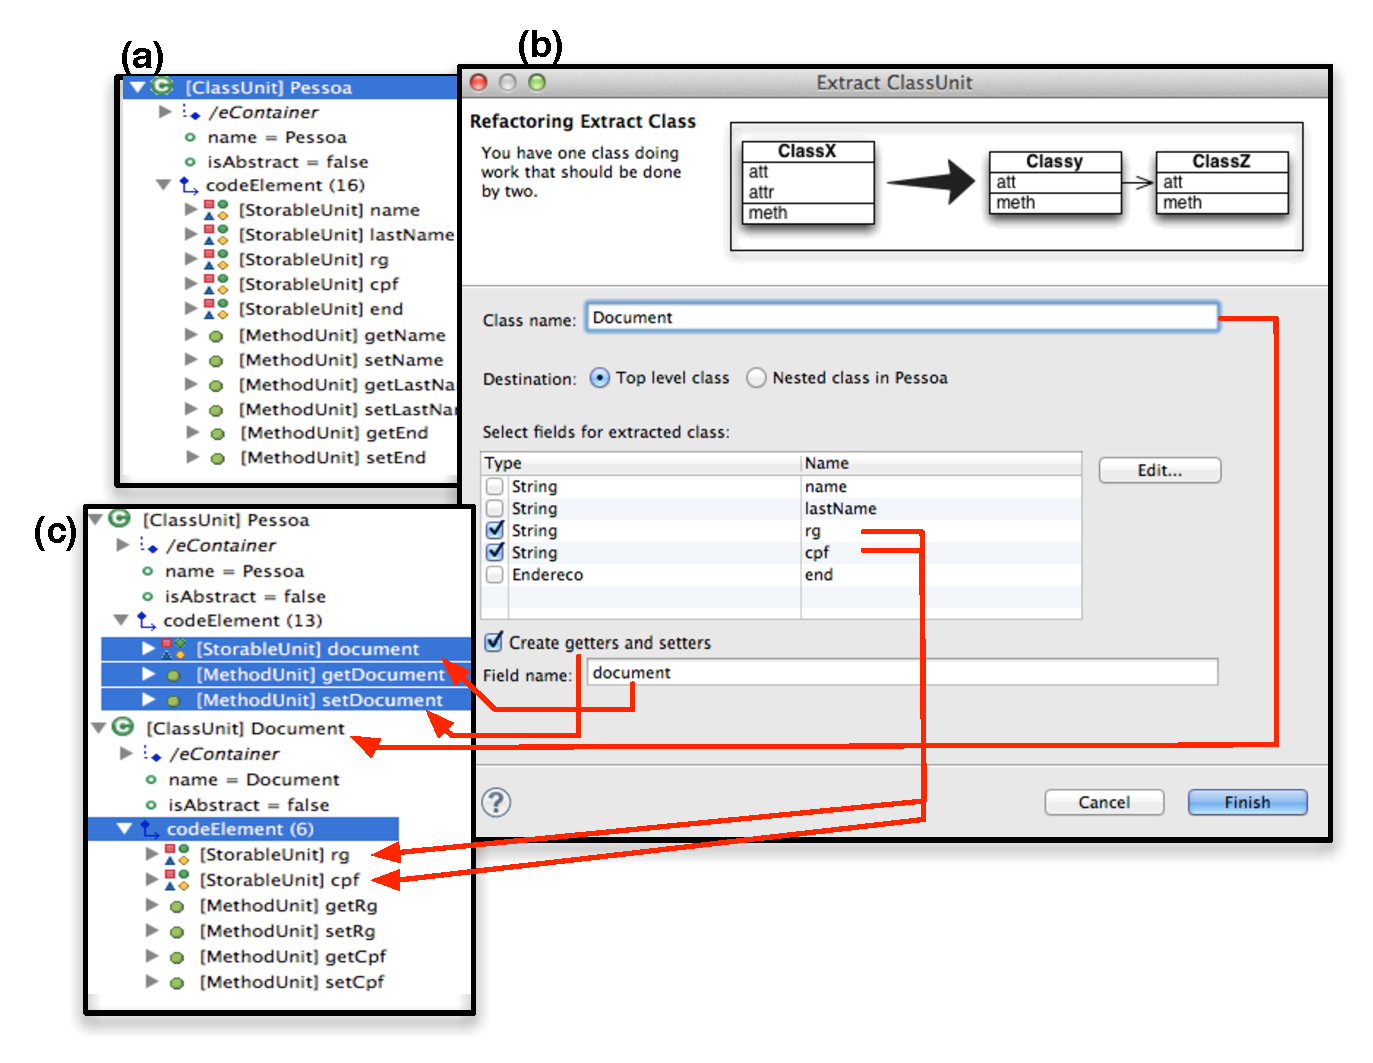
\includegraphics[scale=0.6]{figure/Wizard2}
\caption{Extract Class Wizard}
\label{fig:wizard}
\end{figure}

Notice that KDM-RE also provides a way to indicate refactoring opportunities. Refactoring itself will not bring the full benefits, if we do not understand when refactoring needs to be applied. Thus, to make it easier for the engineer to decide whether certain software needs refactoring or 
not KDM-RE implements a set of bad code smell according to~\cite{bad_smeel_}.

For explanation purpose pretend that the KDM-RE found out that one class is doing work that should be done by two, thus, he must apply the refactoring ``Extract Class''. The first step is to select the metaclass that KDM-RE identified as a bad smell, i.e., the metaclass to be extracted into a separate one, this step is illustrated in Figure~\ref{fig:wizard}(a). After selecting the metaclass, a right-click opens the context menu where the refactoring is accessible. After the click, the system displays the ``RefactoringWizard'' to the engineer, Figure~\ref{fig:wizard}(b) depicts the Extract Class Wizard. In this wizard, the name of the new metaclass can be set. Also a preview of all detected \texttt{StorableUnits} and \texttt{MethodUnits} that can be chosen to put into the new metaclass. Further, the engineer can select if either the new metaclass will be a top level metaclass or a nested metaclass. The engineer also can select if the KDM-RE must create instances of \texttt{MethodUnits} to represent accessors methods (gets and sets). Finally, the engineer can set the name of the \texttt{StorableUnit} that represent the link between the two metaclasses (the old metaclass and the new one). After all of the required inputs have been made, the engineer can click on the button ``Finish'' and the refactoring ``Extract Class'' is performed by KDM-RE. As can be seen in Figure~\ref{fig:wizard}(c) a new instance of \texttt{ClassUnit} named ``Document'' was created - two \texttt{StorableUnit} from ``Pessoa'', i.e., ``rg'' and ``CPF'' were moved to the new \texttt{ClassUnit} - instances of \texttt{MethodUnits} were also created to represent the gets and sets. In addition, the instance of \texttt{ClassUnit} named ``Pessoa'' owns a new instance of \texttt{StorableUnit} that represent the link between both \texttt{ClassUnits}. Due space limitation the other \texttt{StorableUnits} of \texttt{ClassUnit} named ``Pessoa'' are not shown in Figure~\ref{fig:wizard}(c).

After the engineer realize the refactoring a UML class diagram is created on the fly to mirror graphically all changes performed in the KDM model, see Figure~\ref{fig:interface}\textcircled{b}. Moreover, the KDM-RE creates/updates a tracking log to show the historic of all changes performed in the system, as can be see in Figure~\ref{fig:interface}\textcircled{d}. 

\subsection{Forward Engineering}
After the engineer realize the refactoring the next step are to transform the KDM model to a PSM, i.e., a Java Meta-Model and to generate the refactored source-code conforming the PSM. The former step is carried out based on a set of transformations using ATL, due space limitation these transformations are not depicted. Then after transform the KDM to a instance of Java meta-model 

The latter was performed by using a textual template approach, such as the Acceleo\footnote{http://www.eclipse.org/acceleo/}. A template can be thought of as the target text with holes for variable parts. The holes contain metacode which is run at template instantiation time to compute the variable parts. In Figure~\ref{fig:forward_Engineering} the generation of source code using template is depicted.

\begin{figure}[!ht]
\centering
  % Requires \usepackage{graphicx}
  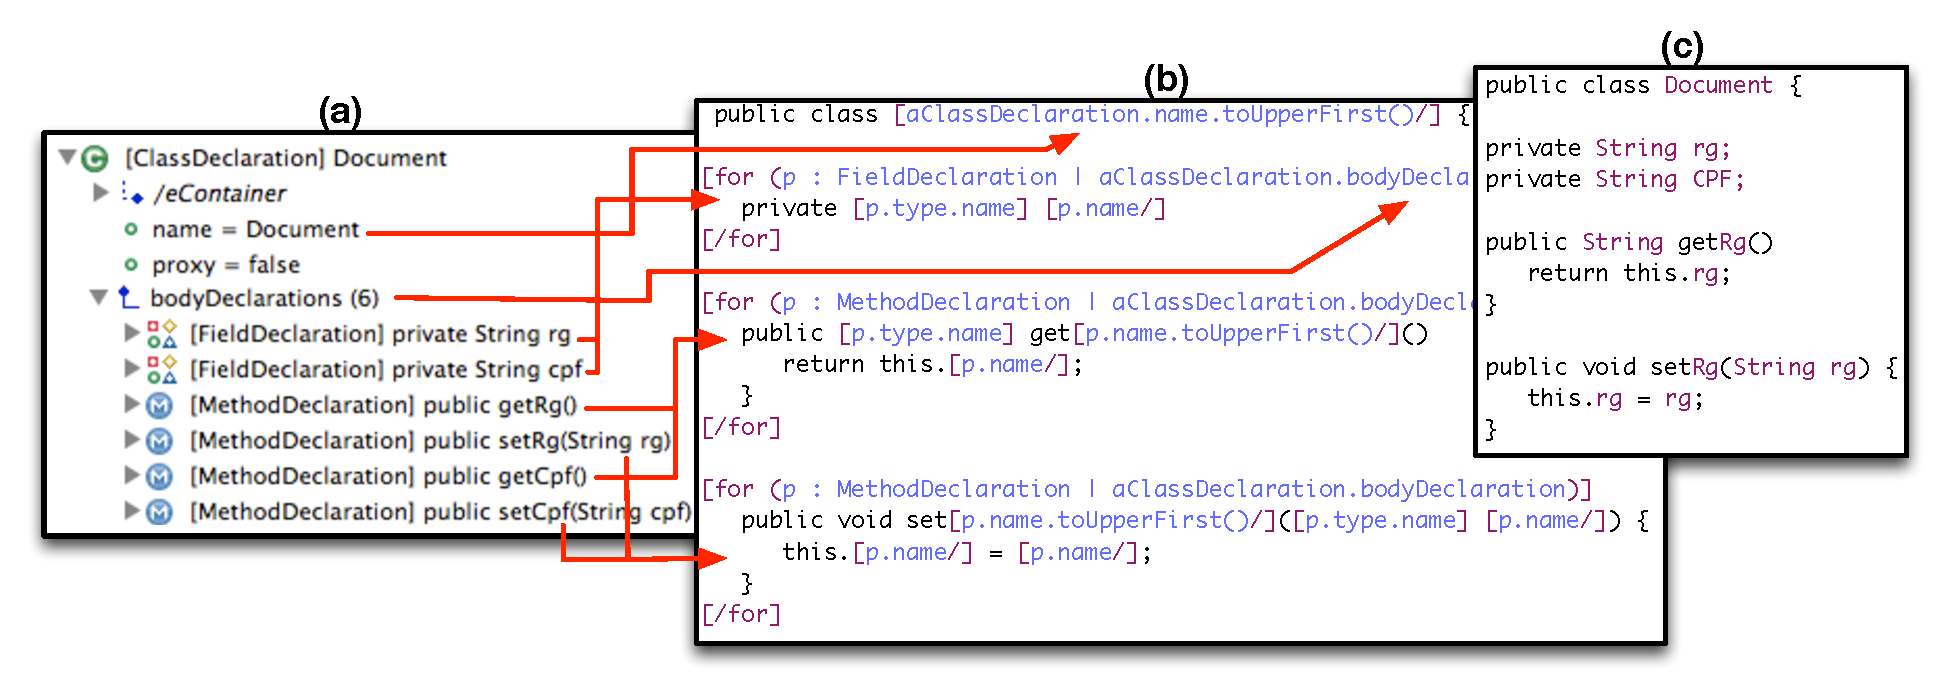
\includegraphics[scale=0.48]{figure/Forward_Engineering2}
\caption{Forward Engineering steps}
\label{fig:forward_Engineering}
\end{figure}

%\subsection{Domain Engineering\label{sec:de}}  
%	%Figure~\ref{fig:proline} depicts a screenshot of ProLine-RM. 
%The DE phase is exhibited by letter ``A'' to ``C'' in Figure~\ref{fig:proline}. 
%In order to illustrated the useful of the ProLine-RM and its functionalities we describe all activities necessaries to devise a ``persistence'' CFF. 
As in development of any framework, firstly the expertise of the domain has to be got.
Therefore, the domain related to ``persistence'' has been studied. 
The outcome of such study were the identification of both the common features and its variants of the domain. 

%After identifying the all features of the CFF the next activity is the development of the CFF. 
In this activity all source code are developed and organized in packages. Each package contain source code (e.g., classes, aspects and methods) related to a feature. %For the purpose of accomplishing this activity we have used the approach described by~\citet{deCamargo:2008:PDC:1363686.1363863}, its aims is to assists and makes easier the develop of the CFF by using aspect oriented paradigm~\cite{Kiczales97aspect-orientedprogramming}. 

Afterwards, the feature model depicting all features related to the domain has to be modeled. 
Aiming to make easier the development of feature models, ProLine-RM provides a graphical way to assists the engineer devises them. 
Figure~\ref{fig:proline}(C) shows the feature model that we have developed. 
As can be seen, there are two set of mandatory features and two groups related to optional features as well.  
%The first one, called ``Persistence'' aims to introduce a set of persistence operations into application persistence classes (e.g., store, remove, update, perform queries). 
%The second feature, named ``Connection'' is related to the database connection concern and identifies points in the application code where the connection must be opened and closed. 
%This feature has variabilities, as for example Data Base Management System (e.g., MySQL, SyBase, Native and Interbase).
%There are two optional features as well. The former is called ``Caching'', which is responsible to deals with high-performance to gets datas of the databases.
%The second, named ``Pooling'' is represented a set of database connections maintained by the databases.

After developing the CFF and the its feature model, them have to be uploaded in a remote repository in order to be reused during the AE phase.
Prior to uploading these artifacts, informations (e.g., Named of CFF, Author(s) and Description) associated with the ``persistence'' CFF has to be filled in. Figure~\ref{fig:proline}(A) shows an example, which the CFF and its feature model are being uploaded. In the next section is described how to reuse the ``persitence'' CFF.

%\subsection{Application Engineering\label{sec:ae}} 
   %%The AE phase is represented by the numbers 1 to 3 as shown in Figure~\ref{fig:proline}. 
%As stated previously, in the AE is wherein the reuse is started effectively.

Firstly, the engineer has to look in the repository and determine whether there are some CFF(s), which can be reused, to make easier and faster the development of the base application. 
In order to assist this activity, ProLine-RM provides a table, which depicts all CFFs that have been uploaded by the engineers in the DE phase.
Figure~\ref{fig:proline}(B) shows this table. 
As can be seen there are six different CFFs - persistence, security, distribution, concurrency, logging and 	Business, respectively. 
In addition, ProLine-RM also shows descriptions for each of the selected CFFs by clicking on the button ``Description''. 
Using this description the engineer can choose the CFFs. 
Nevertheless, if this description is not enough to help the engineer takes a decision on reusing the CFF, ProLine-RM supplies a way visualizes the feature model related to selected CFF by clicking on the button ``View''. 
As is shown in Figure~\ref{fig:proline}(B) the ``persistence'' CFF is highlighted meaning that it has been chosen. 
Next, the ``Download'' button has to be clicked to transfer the feature model belonging to the CFF chosen from the remote repository to the engineer computer.

Secondly, to reuse the CFF its features must be chosen by the engineer aiming to specify explicitly which features will be used in the application base. This is important because usually the CFFs have a great deal of features that probably will not be used in the application base. To assist this activity ProLine-RM uses a file named ``configuration file''. This file is created based on the feature model downloaded. ProLine-RM reads the feature model and creates a ``tree hierarchy''. By using this ``configuration file'' features can be chosen by the engineer. The ``configuration file'' related to the ``persistence'' CFF is shown in Figure~\ref{fig:proline}(D). Moreover, it is interesting to provide a way to validate if the selected features match a valid combination for the instantiation of a member of the CFF, since, certain combinations of features may not lead to useful variants (e.g., in our example the ``persistence'' CFF only a single database connection may be used). ProLine-RM support this validation automatically. As shown in Figure~\ref{fig:proline}(D) once the engineer has chosen the features (represented by ``+''), the resulting variant and constraints are generated automatically (represented by ``-''). 

Finally, the engineer has to submit this validated ``configuration file'' to the remote repository where all CFFs persist. Using this ``configuration file'' the repository will carry out an algorithm. This algorithm aims to extract two artifacts, the codes (e.g., classes, aspects, and packages) related to the features that was chosen by the engineer and a `Reuse Model' (RM), which it is useful to assist the instantiation of CFF's member. After that, these artifacts are sent by the repository to the ProLine-RM. %As can be seen in Figure~\ref{fig:proline}(3) the repository sent only the packages related to the features selected and specified through the ``configuration file'' i.e., the features Persistence, Connection and MySQL.
The application engineer has to filled in the RM. For instance, the value ``base.Custormer.initial'' is a method of the base application and was inserted by the application engineer in the third line of box ``Connection Opening''. After the application engineer fills in the RM with the information needed by an member of a CFF, it is possible to generate the final reuse code.

     
%To the best of our knowledge, there is no an approach that shares, managements, provides full cycle of reuse of the CFF and even supplies a way to examine previously if the features available in one CFF fulfill the application requirements. In order to overcome these absence we put forward an approach and a tool named Proline-RM acronym for Product Line-Repository Manager, which aims to increase the level of manager and accelerate the instantiation of members belonging to a given CFF. The use of the approach is twofold, the Domain Engineering (DE) where all artifacts are developed and upload to a remote server, and the Application Engineering (AE), where the reuse is done effectively. 

\section{Architecture\label{sec:architecture}}
 In Figure~\ref{fig:architecture} is depicted the architecture of KDM-RE which is split in three layers. As shown in this figure, the first layer of our \textit{plug-in} is the Core Framework. This layer represents that  we devised the  \textit{plug-in} on the top of the Eclipse Platform. In this layer it is also possible to see that we  used both Java and Groovy as programming language. Moreover, this layer contains Eclipse Plugins on which our tool is based on, such as MoDisco and EMF. We used MoDisco\footnote{http://www.eclipse.org/MoDisco/} that is an extensible framework to develop model-driven tools to support use-cases of existing software modernization and provides an Application Programming Interface - (API) to easily access the KDM model. Also, Eclipse Modeling Framewokr (EMF)\footnote{http://www.eclipse.org/modeling/emf/} was used to load and navigate KDM models that were generated with MoDisco. 

\begin{figure}[!ht]
\centering
  % Requires \usepackage{graphicx}
  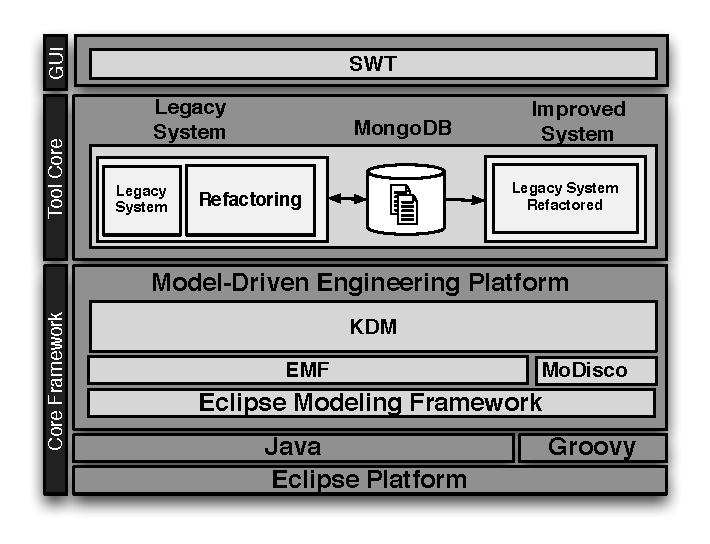
\includegraphics[scale=0.8]{figure/Arquitetura}
\caption{Architecture of KDM-RE}
\label{fig:architecture}
\end{figure}  

The second layer, the Tool Core, is where all refactorings provided by our \textit{plug-in} were implemented. KDM-RE works intensively with KDM models, which are XML files. Therefore, we use Groovy to handle those types of files because of the simplicity of its syntax and fully integrated with Java. KDM-RE also provides a way to create multiple versions of the KDM file to allow the engineer  to assess different refactorings in the same system. In order to optimizes memory usage of multiple versions for large models and enabling to work interactively on multiple models our \textit{plug-in} persists these models in a MongoDB. We chose MongoDB since it provides a high performance. After the engineer to choose a version refactored a forward engineering is carried out and the source code of the modernized target system is generated again. Finally, the top layer is the Graphical User Interface (GUI) that consists of a set of SWT windows with several options to perform the refactorings based on the KDM model.




\section{Related Work\label{sec:related}}
 Borger et al.~\cite{Boger2002} developed a plug-in for the CASE tool ArgoUML that support UML model-based refactorings. The refactoring of class, states and activities is possible, allowing the user to apply refactorings that are not simple to apply at source code level. 
Van Gorp et al.~\cite{Gorp03towardsautomating} proposed a UML profile to express pre and post conditions of source code refactorings using Object Constraint Language (OCL) constraints. The proposed profile allows that a CASE tool: (\textit{i}) verify pre and post conditions for the composition of sequences of refactorings; and (\textit{ii}) use the OCL consulting mechanism to detect bad smells such as crosscutting concerns.

The differential of our approach described herein in relation to the other is the proposal to move from software refactoring to model-driven refactoring by means of KDM, which is a platform and language independent metamodel.


\section{Concluding Remarks\label{sec:conclusion}}
 In this paper is presented the KDM-RE which provides support to model-driven refactoring based on ADM and uses the KDM standard. It follows the theory of the horseshoe modernization model, which is threefold: (\textit{i}) Reverser Engineering, (\textit{ii}) Refactoring and  (\textit{iii}) Forward Engineering. 

Firstly, the engineer starts the refactoring process by means of a KDM file or a source code to be refactored. If the engineer provides a KDM file then KDM-RE can already apply the refactorings. Otherwise, the source code of the legacy system must be transformed into PSMs. Still in the first step, these PSMs are converted into a KDM model through a set of M2M transformation by means of MoDisco. Secondly, the engineer by using KDM-RE can apply a set refactorings in this KDM. Also, on the fly the engineer can check all changes realized in this KDM replicated into a class diagram - the engineer can visually verify the system`s changes after applying a set of refactorings. KDM-RE also supplies a multiple versions of a system at level models. Finally, KDM-RE performs a forward engineering then a refactored source code is generated.

We believe that KDM-RE makes a contribution to the challenges of Software Engineering which focuses on mechanisms to support the automation of model-driven refactoring. Future work involves implementing more refactorings and conducting experiments to evaluate all refactorings provided by KDM-RE. Notice that KDM-RE is open source and it can be downloaded at\textit{~www.dc.ufscar.br/$\sim$valter/KDM-RE}.

\section{Acknowledgements}
 Rafael S. Durelli would like to thank the financial support provided by FAPESP, process number 2012/05168-4. %Bruno Santos and Raphael Honda also would like to thank CNPq for sponsoring our research.

\bibliographystyle{apalike}
\bibliography{referencias}

\end{document}
